\section{Introduction to Embedded Linux}

\begin{frame}{Simplified Linux system architecture}
  \begin{center}
    \includegraphics[height=0.8\textheight]{slides/buildroot-introduction/linux-system-architecture.pdf}
  \end{center}
\end{frame}

\begin{frame}{Overall Linux boot sequence}
  \begin{center}
    \includegraphics[height=0.8\textheight]{slides/buildroot-introduction/overall-boot-sequence.pdf}
  \end{center}
\end{frame}

\begin{frame}{Embedded Linux work}
  \begin{itemize}
  \item {\bf BSP work}: porting the bootloader and Linux kernel,
    developping Linux device drivers.
  \item {\bf system integration work}: assembling all the userspace
    components needed for the system, configure them, develop the
    upgrade and recovery mechanisms, etc.
  \item {\bf application development}: write the company-specific
    applications and libraries.
  \end{itemize}
\end{frame}

\begin{frame}{Complexity of userspace integration}
  \begin{center}
    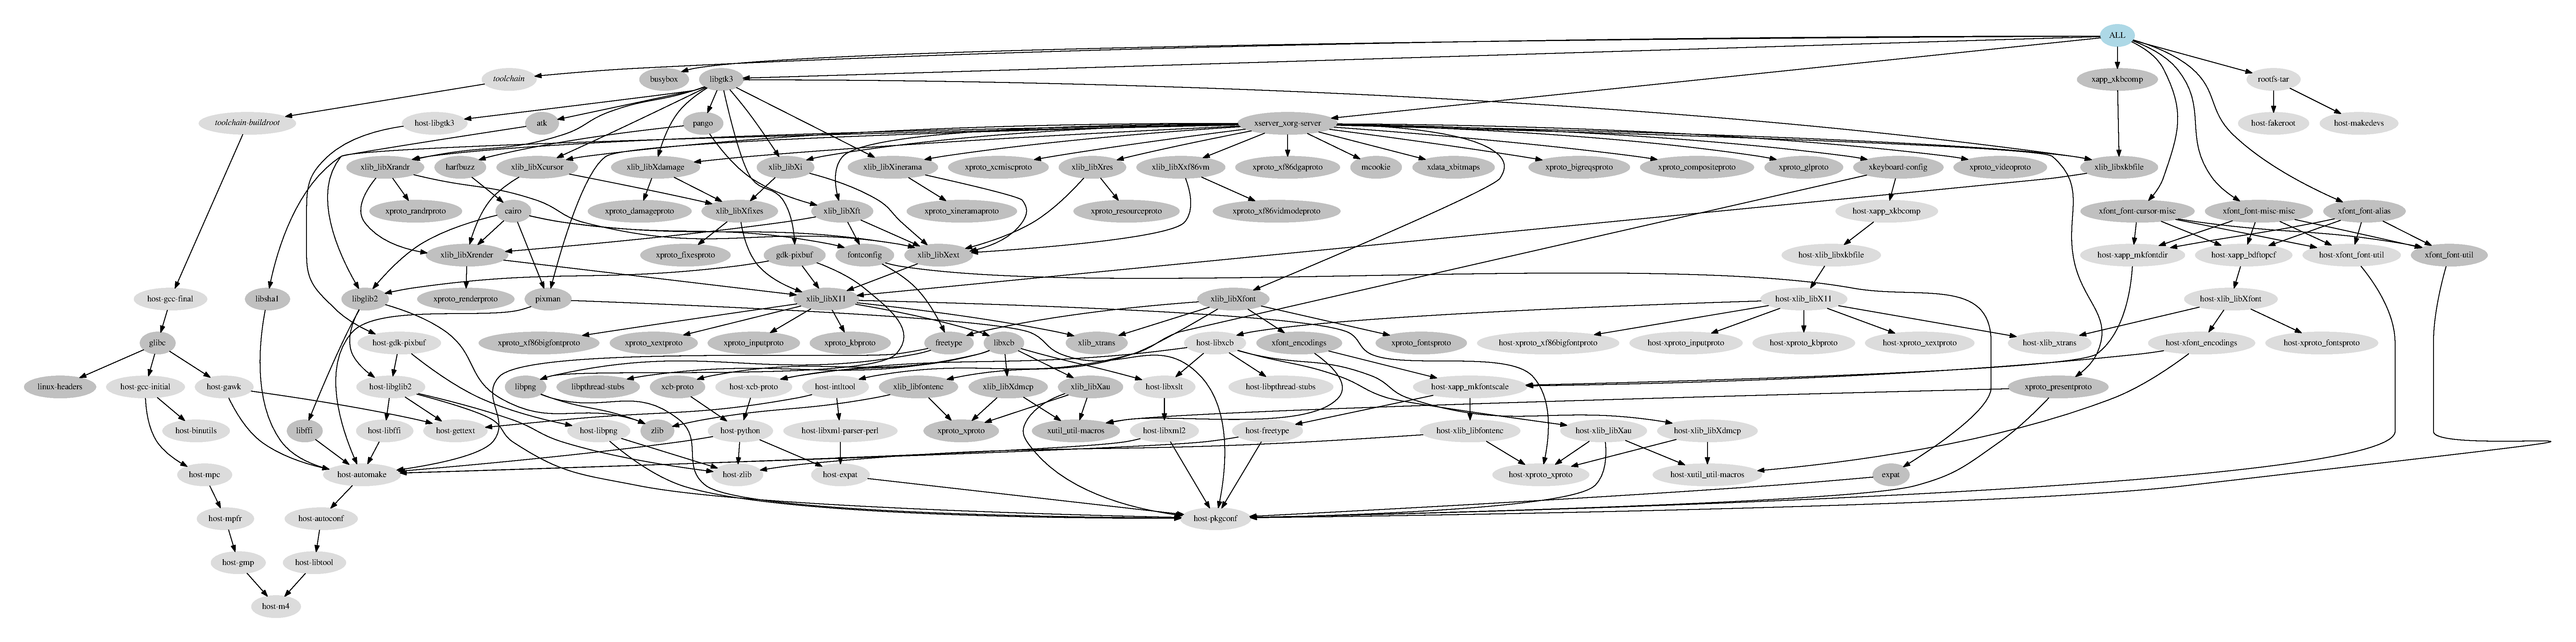
\includegraphics[width=\textwidth]{slides/buildroot-introduction/graph-depends.pdf}
  \end{center}
\end{frame}

\begin{frame}{System integration: several possibilities}
  \scriptsize
  \begin{tabularx}{11cm}{|X|X|X|}
    \hline
    & {\bf Pros} & {\bf Cons} \\
    \hline
    {\bf Building everything manually} &
    Full flexibility \newline
    Learning experience &
    Dependency hell \newline
    Need to understand a lot of details \newline
    Version compatibility \newline
    Lack of reproducitibility \\
    \hline
    {\bf Binary distribution} \newline Debian, Ubuntu, Fedora, etc.
    &
    Easy to create and extend
    &
    Hard to customize \newline
    Hard to optimize \newline
    No way to rebuild the full system from source \newline
    Large system \newline
    Usually slow boot \newline
    Uses native compilation \newline
    Not available for all architectures \\
    \hline
    {\bf Build systems} \newline Buildroot, Yocto, PTXdist, etc.
    &
    Nearly full flexibility \newline
    Built from source: customization and optimization are easy \newline
    Fully reproducible \newline
    Uses cross-compilation
    &
    Not as easy as a binary distribution \newline
    Build time \\
    \hline
  \end{tabularx}
\end{frame}

\begin{frame}{Embedded Linux build system: principle}
  \begin{center}
    \includegraphics[width=0.9\textwidth]{slides/buildroot-introduction/buildsystem-principle.pdf}
  \end{center}
  \begin{itemize}
  \item Building from source $\rightarrow$ lot of flexibility
  \item Cross-compilation $\rightarrow$ leveraging fast build machines
  \item Recipes for building components $\rightarrow$ easy
  \end{itemize}
\end{frame}

\begin{frame}{Embedded Linux build system: tools}
  \begin{itemize}
  \item A wide range of solutions: Yocto/OpenEmbedded, PTXdist,
    Buildroot, LTIB, OpenBricks, OpenWRT, and more.
  \item Today, two solutions are emerging as the most popular ones
    \begin{itemize}
    \item {\bf Yocto/OpenEmbedded}\\Builds a complete Linux
      distribution with binary packages. Powerful, but somewhat
      complex, and quite steep learning curve.
    \item {\bf Buildroot}\\Builds a root filesystem image, no binary
      packages. Much simpler to use, understand and modify.
    \end{itemize}
  \end{itemize}
\end{frame}

\section{Introduction to Buildroot}

\begin{frame}{Buildroot at a glance}
  \begin{itemize}
  \item Can build a toolchain, a rootfs, a kernel, a bootloader
  \item {\bf Easy to configure}: menuconfig, xconfig, etc.
  \item {\bf Fast}: builds a simple root filesystem in a few minutes
  \item Easy to understand: written in make, extensive documentation
  \item {\bf Small} root filesystem, starting at 2 MB
  \item More than {\bf 1500 packages} for userspace libraries/apps available
  \item {\bf Many architectures} supported
  \item {\bf Well-known technologies} : {\em make} and {\em kconfig}
  \item Vendor neutral
  \item Active community, regular releases
  \item \url{http://buildroot.org}
  \end{itemize}
\end{frame}

\begin{frame}{Who's using Buildroot?}
  \begin{columns}
    \column{0.6\textwidth}
    \begin{itemize}
    \item {\bf System makers}
      \begin{itemize}
      \item Google
      \item Barco
      \item Rockwell Collins
      \end{itemize}
    \item {\bf Processor vendors}
      \begin{itemize}
      \item Analog Devices
      \item Imagination Technologies
      \item Marvell
      \item Atmel
      \end{itemize}
    \item Many, many {\bf hobbyists} on development boards:
      Rasberry Pi, BeagleBone Black, etc.
  \end{itemize}
  \column{0.4\textwidth}
  \only{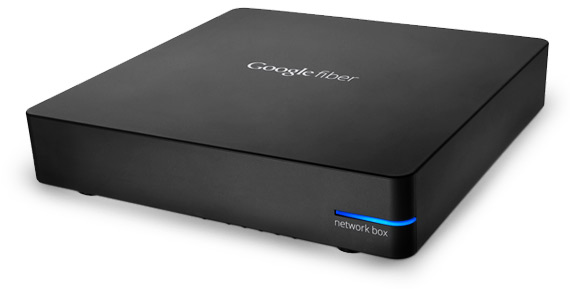
\includegraphics[width=0.8\textwidth]{slides/buildroot-introduction/google-fiber-box.jpg}}\\
  \only{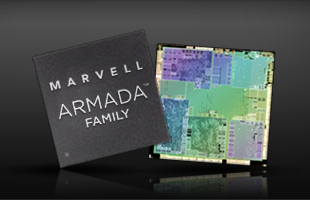
\includegraphics[width=0.8\textwidth]{slides/buildroot-introduction/armada.jpg}}\\
  \only{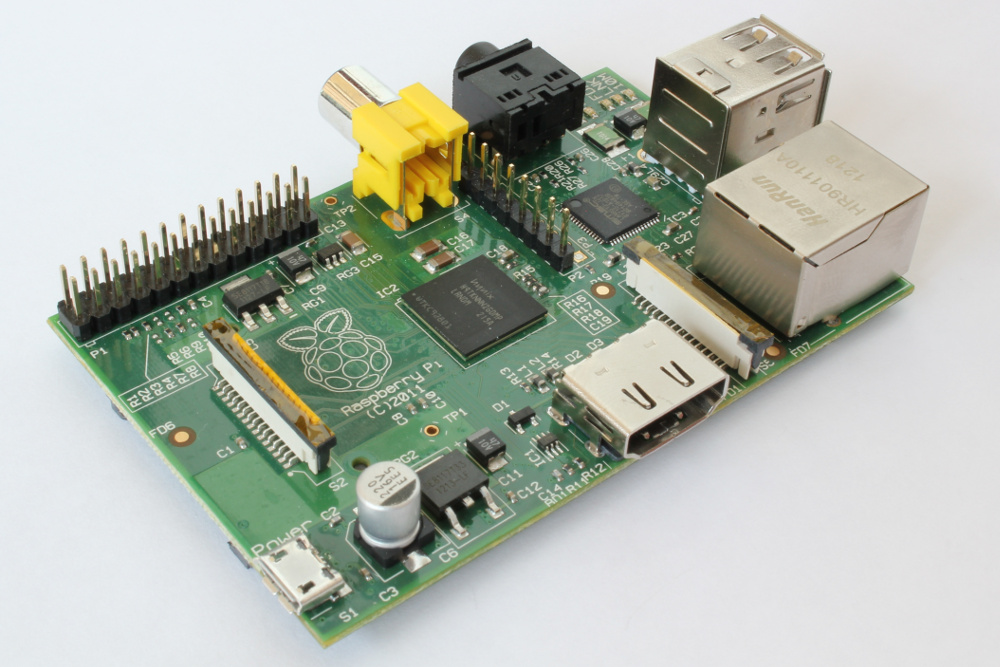
\includegraphics[width=0.8\textwidth]{slides/buildroot-introduction/rasberrypi.jpg}}
  \end{columns}
\end{frame}

\setuplabframe
{Basic Buildroot usage}
{
  \begin{itemize}
  \item Getting and setting up Buildroot
  \item Configuring and building a basic system with Buildroot
  \item Running the system on a hardware platform and in QEMU
  \end{itemize}
}
